% !TEX root = Dokumentation.tex
\subsection{Team}

\begin{figure}[H]

\includegraphics[width=0.4\textwidth]{./04_Projektmanagement/fig/adrianwuersch.jpg}
	\caption{Adrian Würsch}
\end{figure}

\begin{figure}[H]
	
\includegraphics[width=0.4\textwidth]{./04_Projektmanagement/fig/joelmeloni.jpg}
	\caption{Joel Meloni}
\end{figure}

\begin{figure}[H]
	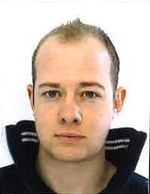
\includegraphics[width=0.4\textwidth]{./04_Projektmanagement/fig/larswalther.jpg}
	\caption{Lars Walther}
\end{figure}

\begin{figure}[H]
	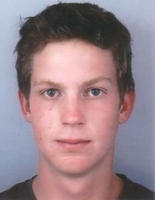
\includegraphics[width=0.4\textwidth]{./04_Projektmanagement/fig/patriziobrantschen.jpg}
	\caption{Patrizio Brantschen}
\end{figure}

\begin{figure}[H]
	
\includegraphics[width=0.4\textwidth]{./04_Projektmanagement/fig/silvanritz.jpg}
	\caption{Silvan Ritz}
\end{figure}

\begin{figure}[H]
	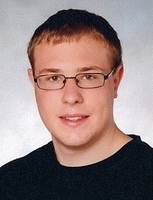
\includegraphics[width=0.4\textwidth]{./04_Projektmanagement/fig/stefanhaefliger.jpg}
	\caption{Stefan Häfliger}
\end{figure}

\begin{figure}[H]
	
\includegraphics[width=0.4\textwidth]{./04_Projektmanagement/fig/tobiaskreienbuehl.jpg}
	\caption{Tobias Kreienbühl}
\end{figure}

